\documentclass{article}


% Set page size and margins
% Replace `letterpaper' with `a4paper' for UK/EU standard size
\usepackage[letterpaper,top=2cm,bottom=2cm,left=3cm,right=3cm,marginparwidth=1.75cm]{geometry}

% Useful packages
\usepackage{amsmath}
\usepackage{graphicx}
\usepackage[colorlinks=true, allcolors=blue]{hyperref}

\title{PS7}
\author{Opal Fraser}

\begin{document}
\maketitle

\section{Questions}
(Preliminary printout is labeled 'PS7 Fraser.docx')
6. At what rate are log wages missing? Do you think the logwage variable is most likely to be MCAR, MAR, or MNAR? 

Answer: 25 percent of log wages are missing. The missingness is not related to any other variables in the data, so it may be MCAR.

7. The true value of ˆb1 = 0.093. Comment on the differences of ˆb1 across the models.
What patterns do you see? What can you conclude about the veracity of the various
imputation methods? Also discuss what the estimates of ˆb1 are for the last two
methods. 

The true value of ˆb1 = 0.093. Comment on the differences of ˆb1 across the models. 
My b1 was the same across the four models. Not sure if I did them correctly or not.

What patterns do you see? hgc, college, and tenure are statistically significant across the four models. If the true value of ˆb1 is 0.093 it is close to b1 = 0.062. We would need to have infinite number of observations in the dataset to produce the exact ˆb1 = 0.093. College and tenure are positive in direction, they have a positive relationship with logwage.

What can you conclude about the veracity of the various imputation methods? 
The imputation methods did not change the answer very much in my estimates. 

Also discuss what the estimates of ˆb1 are for the last two methods. The estimate for b1 in the last two models is 0.062. This suggests that the last two methods are reliable for the data.

\begin{figure}
\centering
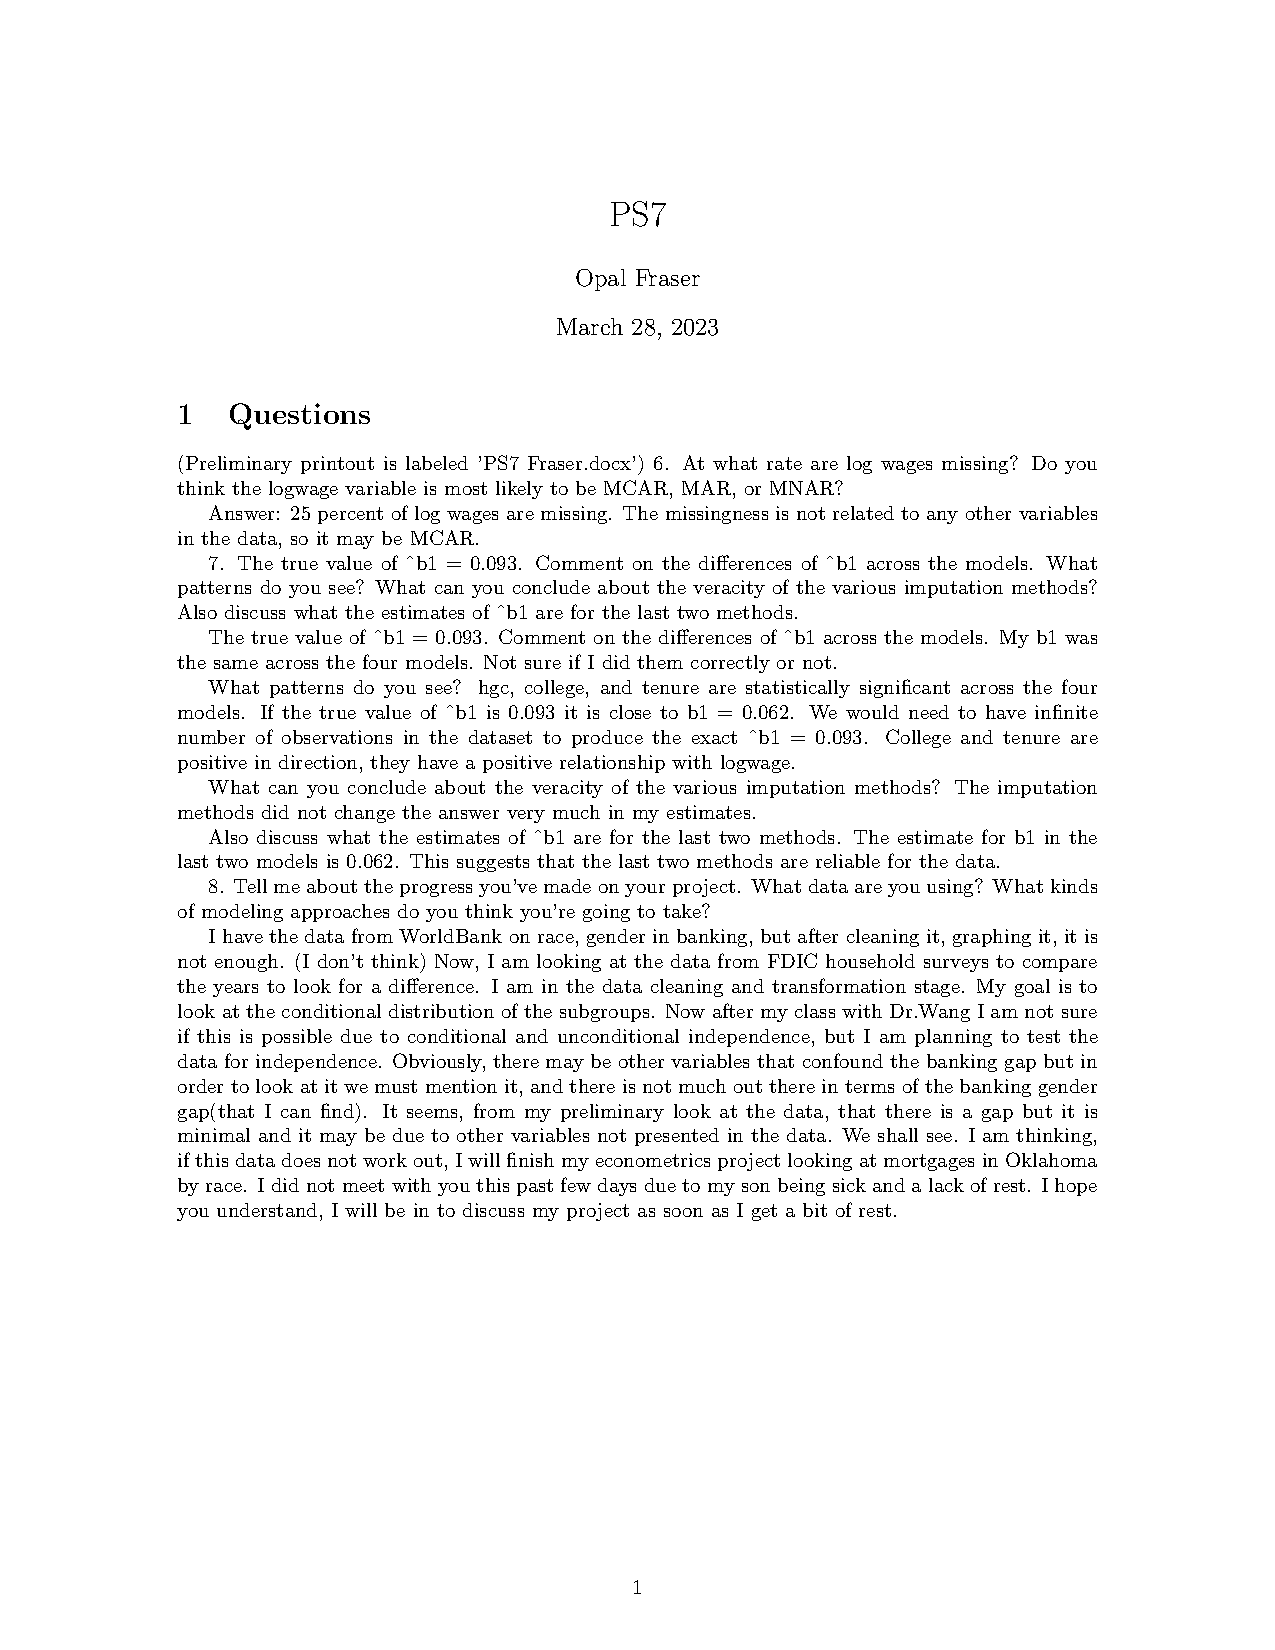
\includegraphics[width=0.9\textwidth]{PS7_Fraser.png}
\caption{\label{fig:PS7_Fraser.png} Model summary with four estimates.}
\end{figure}


8. Tell me about the progress you’ve made on your project. What data are you using?
What kinds of modeling approaches do you think you’re going to take?

I have the data from WorldBank on race, gender in banking, but after cleaning it, graphing it, it is not enough. (I don't think)
Now, I am looking at the data from FDIC household surveys to compare the years to look for a difference. I am in the data cleaning and transformation stage. My goal is to look at the conditional distribution of the subgroups. Now after my class with Dr.Wang I am not sure if this is possible due to conditional and unconditional independence, but I am planning to test the data for independence. Obviously, there may be other variables that confound the banking gap but in order to look at it we must mention it, and there is not much out there in terms of the banking gender gap(that I can find).
It seems, from my preliminary look at the data, that there is a gap but it is minimal and it may be due to other variables not presented in the data. We shall see. 
I am thinking, if this data does not work out, I will finish my econometrics project looking at mortgages in Oklahoma by race. I did not meet with you this past few days due to my son being sick and a lack of rest. I hope you understand, I will be in to discuss my project as soon as I get a bit of rest. 

\end{document}